\documentclass{beamer}
\usepackage{defs}
\usepackage{tikz-cd}
\usepackage[all,cmtip]{xy}
%
% Choose how your presentation looks.
%
% For more themes, color themes and font themes, see:
% http://deic.uab.es/~iblanes/beamer_gallery/index_by_theme.html
%
\mode<presentation>
{
    \usetheme{CambridgeUS}      % or try Darmstadt, Madrid, Warsaw, ...
    \usecolortheme{default} % or try albatross, beaver, crane, ...
    \usefonttheme{default}  % or try serif, structurebold, ...
    \setbeamertemplate{navigation symbols}{}
    \setbeamertemplate{caption}[numbered]
} 

\newcommand{\indexset}{\mathcal{I}}
\newcommand{\fourcoeff}[3]{\ensuremath{F^{#3}_{(#1,#2)}}}
\DeclareMathOperator{\det}{det}
\DeclareMathOperator{\adj}{adj}
\DeclareMathOperator{\len}{len}
\DeclareMathOperator{\real}{Re}
\DeclareMathOperator{\imag}{Im}
\newtheorem{remark}[theorem]{Remark}
\usepackage[english]{babel}
\usepackage[utf8]{inputenc}
\usepackage[T1]{fontenc}

%\title[Biparametric Persistence]{Biparametric Persistence for Phase space Topology Inference}
\title[Classifying Spaces]{Classifying Spaces for Analysis of Dynamical Systems}
\author[Mishal Assif]{Mishal Assif P K \\ Advisor: Prof. Yuliy Baryshnikov}
\institute[ECE]{Electrical and Computer Engineering, UIUC}
\date{\today}

\AtBeginSection[]
{
    \begin{frame}
        \frametitle{Table of Contents}
        \tableofcontents[currentsection]
    \end{frame}
}
%\newcommand{\Var}{\mathrm{Var}}
\newcommand{\Var}[1]{\ensuremath{\mathsf{Var}\!\left[\vphantom{\big|}#1\vphantom{\big|}\right]}}
\begin{document}


\begin{frame}
    \titlepage
\end{frame}

% Uncomment these lines for an automatically generated outline.
%\begin{frame}{Outline}
%  \tableofcontents
%\end{frame}

\section{Introduction}
\begin{frame}{Introduction}
    \begin{itemize}
        \item Algebraic topology: Studying continuous topological spaces using discrete algebraic descriptors %\pause
        \item Topological data analysis: Computational pipelines using abstract constructions
            for inferring topology from data \pause
        \item Dynamical Systems: 
            \begin{enumerate}
                \item Phase space: $M$ 
                \item Vector field: \ $x(t) \in M, \ \dot{x}(t) = h(x(t))$
                \item Observation function: $g : M \rightarrow \R^n$
    \end{enumerate}
    \pause
\item \textit{Can we recover the topology of the phase space $M$ from trajectories of observations $g(x(t))$ of the dynamical system?}
    \end{itemize}
\end{frame}

\section{Classical Construction \& Desideratum}
\begin{frame}{Classical Construction (CJS approach)}
        \begin{minipage}[b]{0.4\linewidth}
    \begin{itemize}
        \item<1-> $M$ a manifold, $f$ a Morse function and the gradient vector field $\dot{x}(t) = \nabla f(x)$ 
        \item<2-> This gradient flow defines a combinatorial construction (the classifying space 
            of a category) describing the underlying 
            phase space of the system 
        \item<3-> The category consists of critical points, with morphisms that are themselves
            topological spaces of trajectories 
    \end{itemize}
        \end{minipage}
        \hspace{0.5cm}
        \begin{minipage}[b]{0.4\linewidth}
            \begin{figure}
            \includegraphics[width=0.9\textwidth]{../images/morse.png}
            %\caption{PD of Cech filtration of the point cloud in Figure \ref{fig1}}.
            \end{figure}
        \end{minipage}
\end{frame}
\iffalse
\begin{frame}{Classical Construction (CJS approach)}
    \begin{itemize}
        \item $M$ a manifold, $f$ a Morse function and the gradient vector field
            \[
                \dot{x}(t) = \nabla f(x)
            \]
    \end{itemize}
        \pause
        \begin{figure}
        \includegraphics[width=0.3\textwidth, height=0.4\textwidth]{../images/morse.png}
        %\caption{PD of Cech filtration of the point cloud in Figure \ref{fig1}}.
        \end{figure}
\end{frame}
\fi

\begin{frame}{Desideratum}
    Need to port the CJS approach to experimental data:
    \begin{enumerate}
        \item Trajectories obtained need not be from gradient systems
            \[ x \in M, \dot{x} = h(x) \]
            \pause
        \item Typically have access to observations only, not necessarily embeddings
            \[ g : M \rightarrow \R^n \]
            \pause
        \item We can access only a finite number of trajectories
    \end{enumerate}
\end{frame}
\begin{frame}{Desideratum}
    \begin{itemize}
        \item Good news: the underlying theory remains correct under appropriate restrictions
            \pause
        \item The classifying space of the category of trajectories of a general dynamical system
            is homotopy equivalent to the phase space
            \pause
        \item Restriction: no cycles (the pieces of trajectories need to be short enough)
            \pause
        \item Challenge: need to compute the topology of the space of short segments from a finite sample
            \pause
        \item Solution: \textit{Persistent homology}
    \end{itemize}
\end{frame}

\section{Persistent Homology}
\begin{frame}{Topology inference from point clouds}
    \begin{figure}[H]
        \begin{overprint}
            \onslide<1>\centering\includegraphics[width=8cm]{../persist_ex/point_cloud.png}
            \onslide<2>\centering\includegraphics[width=8cm]{../persist_ex/pc_cech1.png}
            \onslide<3>\centering\includegraphics[width=8cm]{../persist_ex/pc_cech2.png}
            \onslide<4>\centering\includegraphics[width=8cm]{../persist_ex/pc_cech3.png}
            \onslide<5>\centering\includegraphics[width=8cm]{../persist_ex/pc_cech4.png}
        \end{overprint}
        \caption{2D Point Cloud}
        \label{fig1}
    \end{figure}
\end{frame}
\begin{frame}{Persistence Diagram}
        \begin{minipage}[b]{0.4\linewidth}
            \begin{figure}
            \includegraphics[width=\textwidth]{../persist_ex/persist.png}
            \caption{PD of Cech filtration of the point cloud in Figure \ref{fig1}}.
            \end{figure}
        \end{minipage}
        \hspace{0.5cm}
        \begin{minipage}[b]{0.4\linewidth}
            \begin{itemize}
            \item Multiscale topology of a point cloud can be completely represented using a concise, discrete descriptor called \textbf{Persistence diagram (PD)} or \textbf{barcode}
            \pause
            \item A point $(b, d)$ in it represents an $n$-dimensional hole 
            in the filtration that was born at time $t = b$ and dies at time $t = d$
            \pause
            \end{itemize}
        \end{minipage}
\end{frame}

\begin{frame}{Computational Pipeline}
    \begin{enumerate}
        \item Generate a sample of observations of trajectories
        \pause
        \item Identify the proximity of subsegments
        \pause
        \item Construct a filtered simplicial complex
        \pause
        \item Compute persistent homology
    \end{enumerate}
\end{frame}

\iffalse
\begin{frame}{Persistence Diagram}
    \begin{figure}[H]
        \begin{center}
            \includegraphics[height=6cm,width=10cm]{../persist_ex/persist.png} 
            \caption{PD of Cech filtration of the point cloud in Figure \ref{fig1}}.
            \label{fig:I2O}
        \end{center}
    \end{figure}
\end{frame}
\fi
\section{Examples}

\begin{frame}{Geodesics on the sphere}
    \begin{itemize}
        \item $M = S^2 \subset \R^3$, \pause 
        \item $\beta_0(M) = 1, \beta_2(M) = 1$, \pause
        \item Segments of geodesics on the sphere corrupted by noise
    \end{itemize}
    \begin{figure}
    \includegraphics[width=0.5\textwidth]{../images/sphere_crop.png}
    %\caption{PD of Cech filtration of the point cloud in Figure \ref{fig1}}.
    \end{figure}
\end{frame}
\begin{frame}{Geodesics on the sphere}
        \begin{figure}
        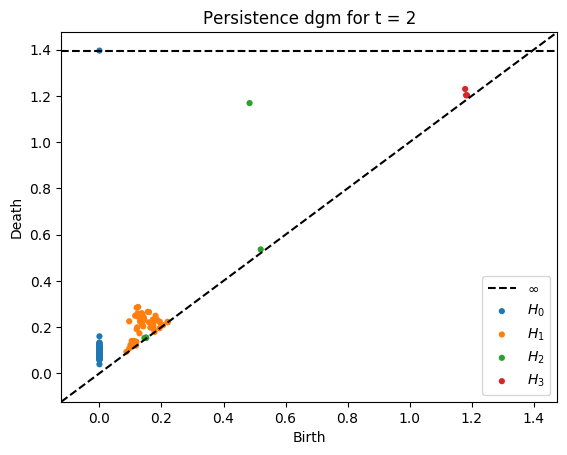
\includegraphics[width=0.6\textwidth]{../images/sphere_pdgm.png}
        \caption{Persistence diagram generated from noisy geodesics on the sphere}.
        \end{figure}
\end{frame}

\begin{frame}{Random vector fields on the 2-Torus}
    \begin{itemize}
        \item $M = S^1 \times S^1 \subset \R^3$, \pause 
        \item $\beta_0(M) = 1, \beta_1(M) = 2, \beta_2(M) = 1$, \pause
        \item 
            \begin{align*}
                \dot{\theta_1}(t) &= \sum_{i=0}^{2} \sum_{j=0}^{2} a_{{i,j}} (i+1)\sin((i+1)\theta_1)\sin((j+1)\theta_2) \\ 
                \dot{\theta_2}(t) &= \sum_{i=0}^{2} \sum_{j=0}^{2} a_{{i,j}} (j+1)\cos((i+1)\theta_1)\cos((j+1)\theta_2)
            \end{align*}
            where $a_{{i,j}}$ are random variables.
    \end{itemize}
\end{frame}

\begin{frame}{Random vector fields on the 2-Torus}
        \begin{minipage}[b]{0.5\linewidth}
            \begin{figure}
            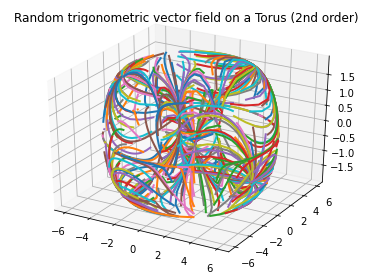
\includegraphics[width=\textwidth]{../images/torus_2.png}
            \caption{Segments of trajectories of random vector field on 2-torus}.
            \end{figure}
        \end{minipage}
        \hspace{0.5cm}
        \pause
        \begin{minipage}[b]{0.4\linewidth}
            \begin{figure}
            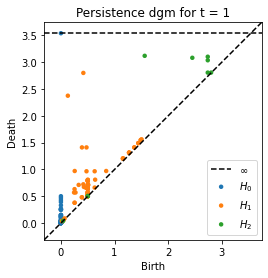
\includegraphics[width=\textwidth]{../images/torus_2_pdgm.png}
            \caption{Persistence diagram generated from these segments}.
            \end{figure}
        \end{minipage}
\end{frame}

\begin{frame}{Random vector fields on the 2-Torus}
        \begin{minipage}[b]{0.5\linewidth}
            \begin{figure}
            \includegraphics[width=\textwidth]{../images/torus_2_obs.png}
            \caption{Segments of observations of trajectories of random vector field on 2-torus}.
            \end{figure}
        \end{minipage}
        \hspace{0.5cm}
        \pause
        \begin{minipage}[b]{0.4\linewidth}
            \begin{figure}
            \includegraphics[width=\textwidth]{../images/torus_2_obs_pdgm.png}
            \caption{Persistence diagram generated from these segments}.
            \end{figure}
        \end{minipage}
\end{frame}

\begin{frame}{Lorenz System}
    \begin{itemize}
        \item Lorenz System:
            \begin{align*}
                \dot{x}(t) &= \sigma(y-x), \\
                \dot{y}(t) &= x(\rho-z) - y, \\
                \dot{z}(t) &= xy - \beta z.
            \end{align*}
            \pause
        \item Chaotic solutions of the Lorenz system form the butterfly shaped Lorenz attractor
    \end{itemize}
\end{frame}

\begin{frame}{Lorenz System}
        \begin{minipage}[b]{0.5\linewidth}
            \begin{figure}
            \includegraphics[width=\textwidth]{../images/lorenz_crop.png}
            \caption{Segments of trajectories of the Lorenz system}.
            \end{figure}
        \end{minipage}
        \hspace{0.5cm}
        \pause
        \begin{minipage}[b]{0.4\linewidth}
            \begin{figure}
            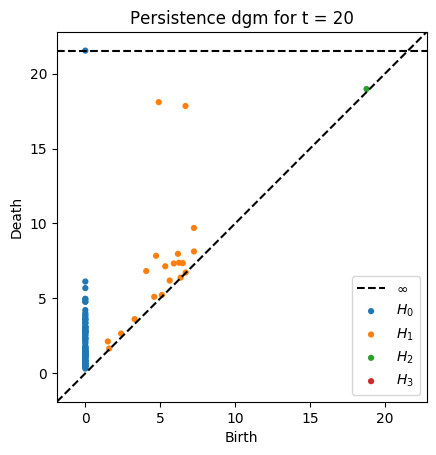
\includegraphics[width=\textwidth]{../images/lorenz_pdgm.png}
            \caption{Persistence diagram generated from these segments}.
            \end{figure}
        \end{minipage}
\end{frame}
\begin{frame}{Lorenz System}
        \begin{minipage}[b]{0.5\linewidth}
            \begin{figure}
            \includegraphics[width=\textwidth]{../images/lorenz_hd.png}
            \caption{Segments of observations of trajectories of the Lorenz system}.
            \end{figure}
        \end{minipage}
        \hspace{0.5cm}
        \pause
        \begin{minipage}[b]{0.4\linewidth}
            \begin{figure}
            \includegraphics[width=\textwidth]{../images/lorenz_hd_pdgm.png}
            \caption{Persistence diagram generated from these segments}.
            \end{figure}
        \end{minipage}
\end{frame}

\begin{frame}{}
    \begin{center}
\Huge Thank You!
\end{center}

\end{frame}
\end{document}

